% !TEX root = ../../thesis.tex

\newpage
\section{Extending Poppy’s sensor apparatus} % (fold)
\label{sec:morphology-adding-mechanism}


Poppy has been designed following a methodology (presented in section~\ref{REF}) which makes hacking the platform easy. With its 3D-printed structure, it is quite easy and straightforward to modify its mechanical parts. Unfortunately we cannot (yet) print complex electronics circuits and components. We therefore chose to fork the Arduino Due board and design a custom I/O board (detailed in section~\ref{REF}). As its name suggests, the main purpose of this board is to manage the several inputs/outputs of the robot and offers:
\begin{itemize}
    \item 2 Dynamixel buses (TTL),
    \item 2 internal USB and 2 external USB ports,
    \item analog and digital pins available on a classic Arduino Due which can be use as direct input/output or for communication buses such as UART, I2C or SPI.
\end{itemize}
Thus there are many more I/Os than required for Poppy. These extra ports are intended to allow Poppy users extend its sensorimotor space and adapt it to their needs.


During our first trials to design walking a primitive with Poppy, we were interested in measuring the under-foot pressure, but the simple foot design Poppy has does not involve appropriate sensors. With a traditional robotic platform, we would have had to either use the available sensors, in this case the load measurement in the ankle Dynamixel motor, or add an external device with its own power supply and communication system.

With Poppy’s electronic modularity, we can hack the robot and integrate new sensors. Then they can be plugged on the I/O board for communication and power supply needs.

To provide an example of how we can actually hack the Poppy robot, we will explain here what we did to integrate force sensors under the feet and acquire the data with the pypot library.

\subsection{Principles} % (fold)
To obtain measurements of the pressure variation under our Poppy's feet we used FSR sensors from Interlink Electronics (see \figurename~\ref{fig:FSR_explode_view}). The FSR sensor will vary its resistance depending on how much pressure is being applied to the sensing area. The harder the force, the lower the resistance is. These sensors are low-cost <\$6 each - yet their behavior is very non-linear (see \figurename~\ref{fig:foot_sensor_behavior}) and the calibration is quite variable depending on the production batch and the thermal conditions. So we cannot expect to obtain precise results.

\begin{figure}[h]
\centering
    \subfloat[][Exploded view\footnote{Illustration credit: \url{http://www.openmusiclabs.com/learning/sensors/fsr/}} of a FSR sensor]{\label{fig:FSR_explode_view}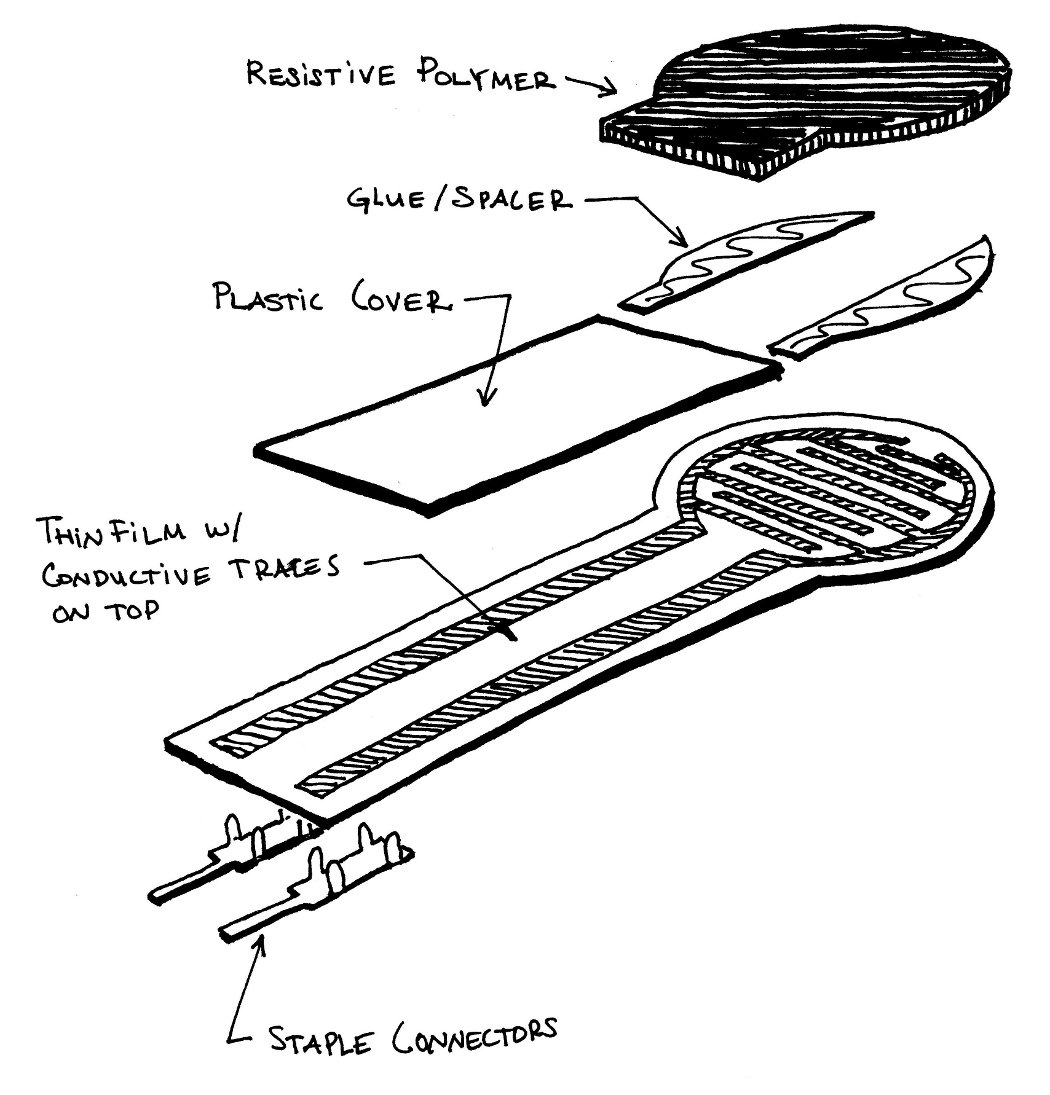
\includegraphics[height=6.3cm]{FSR_explode_view.jpg}}
    \hfil
    \subfloat[][Measured FSR sensor resistance in relation to the applied force.]{\label{fig:FSR_behavior}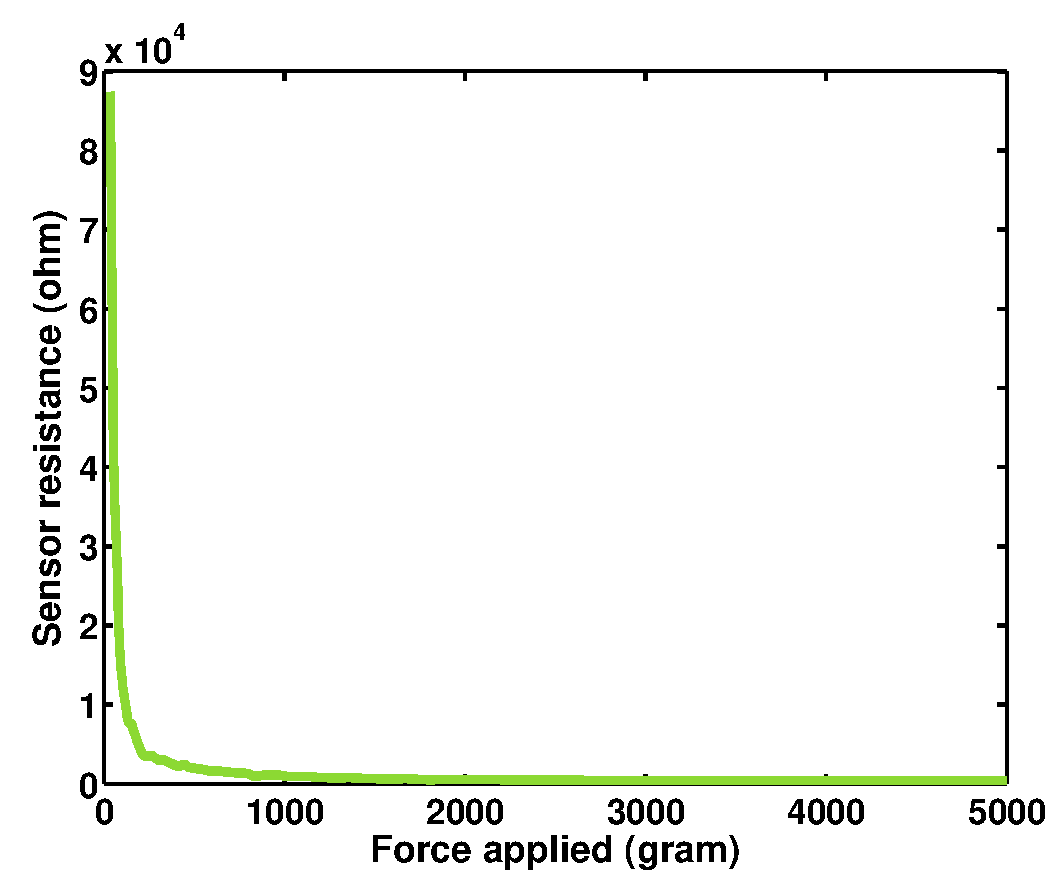
\includegraphics[height=6.3cm]{FSR_behavior.pdf}}
    \caption{The FSR force sensors are cheap but they have very non-linear behavior and are not very precise.}
    \label{fig:}
\end{figure}

The acquisition of the resistance can be done indirectly by designing a voltage-divider\footnote{A voltage divider is a linear circuit that produces an output voltage $V_{out}$ that is a fraction of its input voltage $V_{in}$. It often consists of 2 resistors in series.} and using the FSR resistance variations to vary the voltage output (see \equationname~\ref{eq:voltage-divider}). This voltage ($V_{out}$) can be then measured by an analog input of an Arduino board (see \figurename~\ref{fig:foot_sensors_test}).

\begin{equation}
    V_\mathrm{out} = \frac{R}{R+R_\mathrm{FSR}} \cdot V_\mathrm{in}
\label{eq:voltage-divider}
\end{equation}


\begin{figure}[!h]
\centering
    \subfloat[][A FSR sensor connected with an Arduino nano board.]{\label{fig:foot_sensors_test}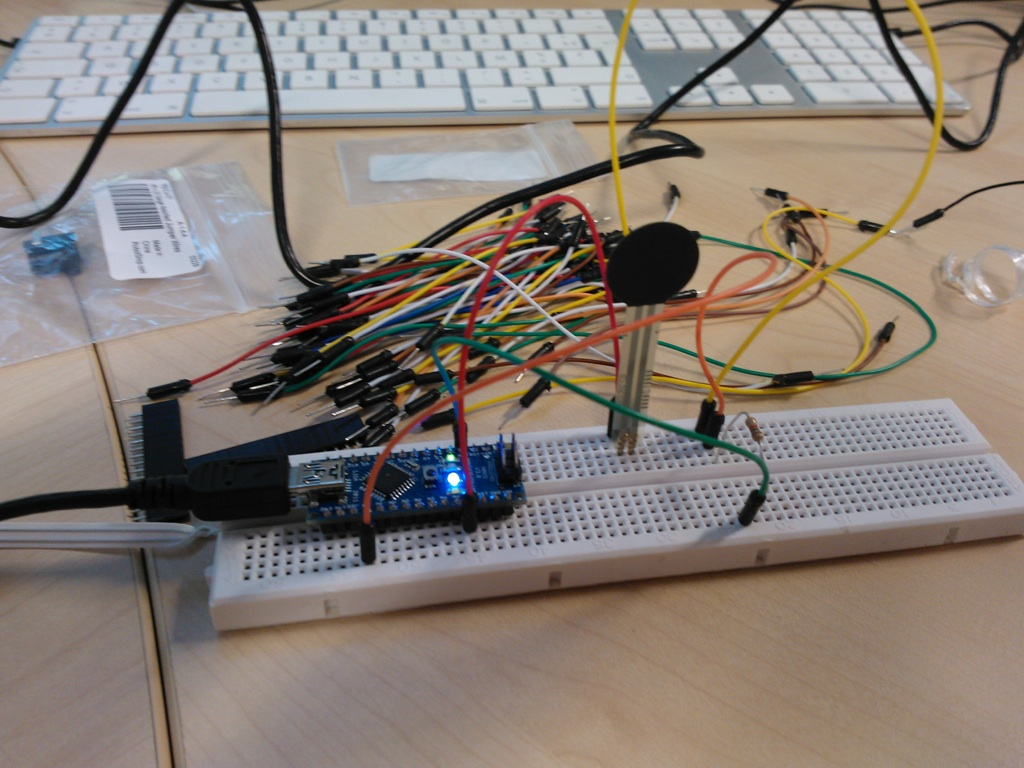
\includegraphics[height=5cm]{force_sensors_test.jpg}}
    \hfil
    \subfloat[][Simple testing assembly with 4 voltage dividers with FSR sensors and potentiometers plugged onto an Arduino nano board]{\label{fig:}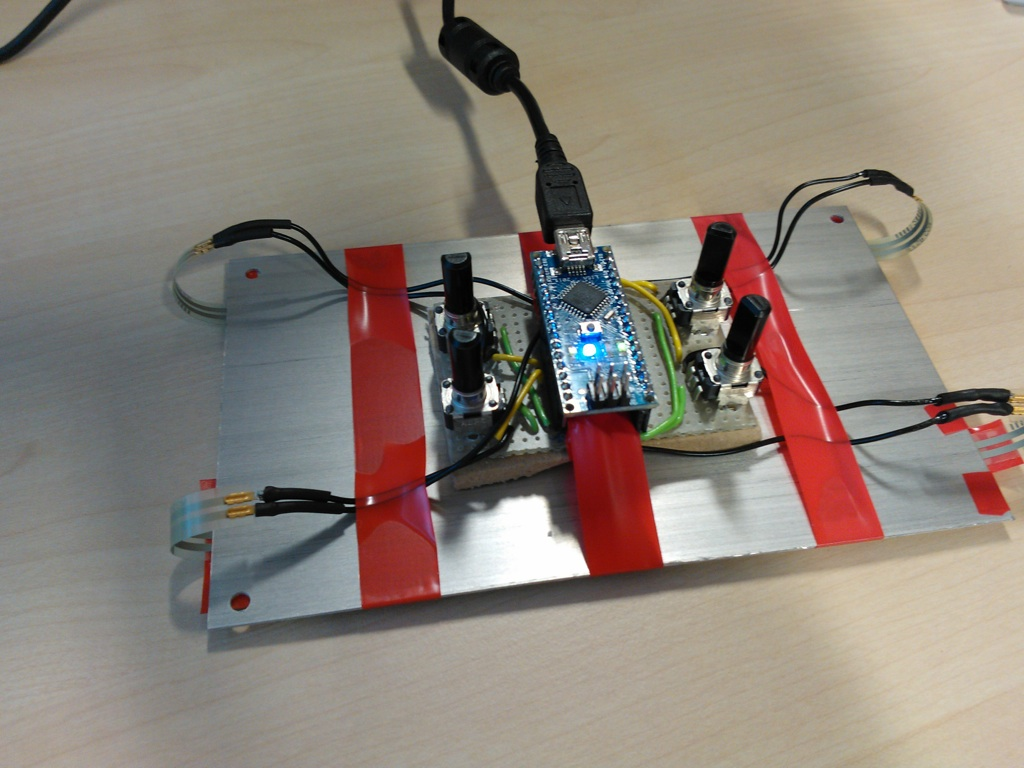
\includegraphics[height=5cm]{foot_sensors_proto.jpg}}
    \caption{We can easily measure the resistance variation of a FSR sensor using a voltage divider with the $V_{out}$ connected to an Arduino analog port.}
    \label{fig:test_sensors}
\end{figure}

\subsection{Design of the voltage divider to reduce the non-linearity of the sensors } % (fold)

% subsection design_of_the_voltage_divider_to_reduce_the_non_linearity (end)
A well-tuned voltage-divider can help to reduce the non-linearity of the FSR sensors. Thus we conducted an optimization of the constant resistor choice depending on:
\begin{itemize}
    \item the Arduino analog precision: $1024$ values for a $5V$ input range,
    \item the use of the Dynamixel tension as voltage input i.e. $14V$,
    \item the standard resistor E12 precision series,
\end{itemize}

With an objective function set to minimize the difference between the actual voltage-divider behavior and the perfect linear behavior $V_\mathrm{out}(F) = \alpha \cdot F$ with $V_\mathrm{out}(3.5kg) = 5V$ (see red curve on \figurename~\ref{fig:obtained_FSR_behavior}), we obtained the $180\Omega$ resistor as the optimal choice, on the basis of the constant resistance of the voltage divider (see \figurename~\ref{fig:FSR_best_resistor}). The best behavior found is plotted in blue in \figurename~\ref{fig:obtained_FSR_behavior}.

\begin{figure}[h]
\centering
    \subfloat[][Optimization of the voltage divider constant resistor: distance between the output behavior with respect to a linear behavior.]{\label{fig:FSR_best_resistor}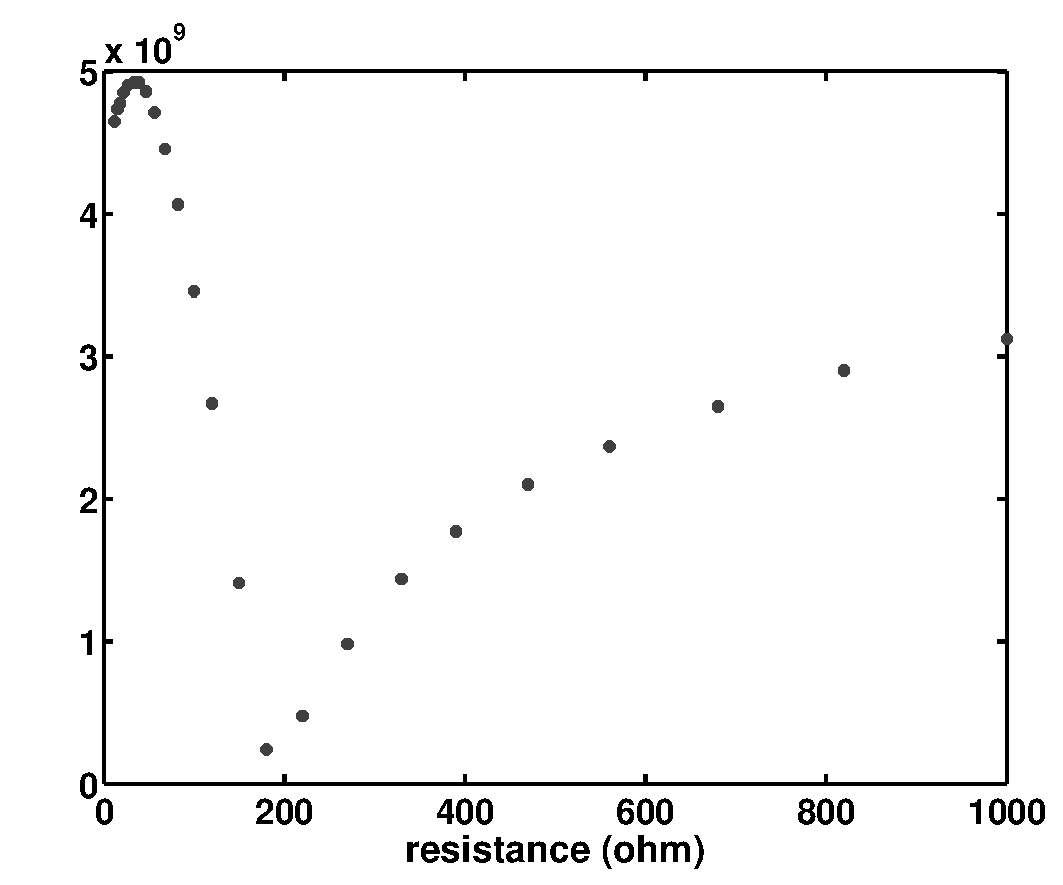
\includegraphics[width=0.48\linewidth]{criteria_dist.pdf}}
    \hfil
    \subfloat[][Theoretical behavior (blue) of the output voltage with respect to the applied force with a $14v$ input and a $180\Omega$ compared with the objective linear behavior.]{\label{fig:obtained_FSR_behavior}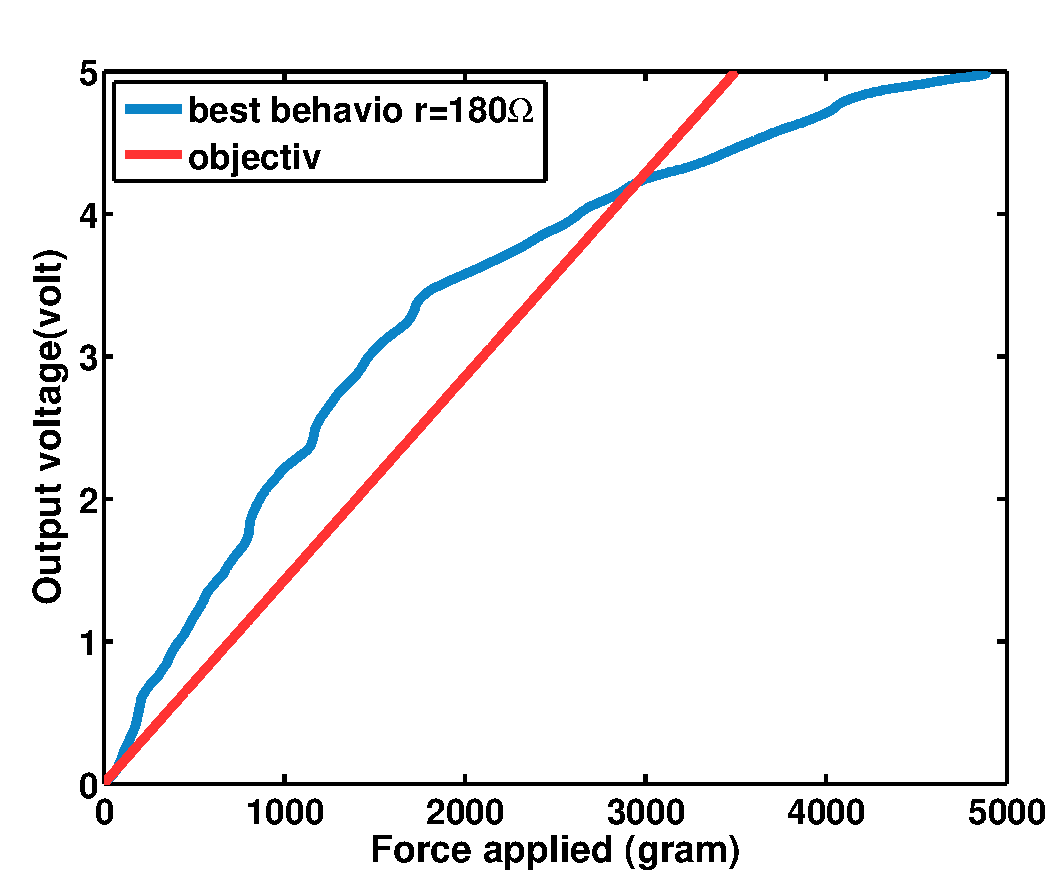
\includegraphics[width=0.48\linewidth]{voltage_behavior.pdf}}
    \caption{The design of the voltage divider for each FSR sensor is done by optimizing the output behavior toward a ideal linear behavior.}
    \label{fig:foot_sensor_behavior}
\end{figure}



\subsection{Integration of foot pressure sensors on Poppy} % (fold)

When we integrated the foot sensors on Poppy, its feet were still a really simple and flexible 3D-printed part. The actual force transmission was done by the shoes. We therefore had to directly attach the sensors below the shoes. Because Arduino nano board has 8 analog inputs, we have added 8 sensors under each foot (see \figurename~\ref{fig:poppy_foot_sensors}) but actually only used 5 (the big ones) and integrated the Arduino nano in the leg. While it was a hack of a real shoe and not just a print of new part, the intervention was rather cumbersome but still achievable in one day. Here we have chosen to use USB cable to plug each Arduino nano in the Poppy's head but it could also have be done using UART, SPI or I2C communication.

\begin{figure}[h]
\centering
    \subfloat[][]{\label{fig:poppy_foot_sensors}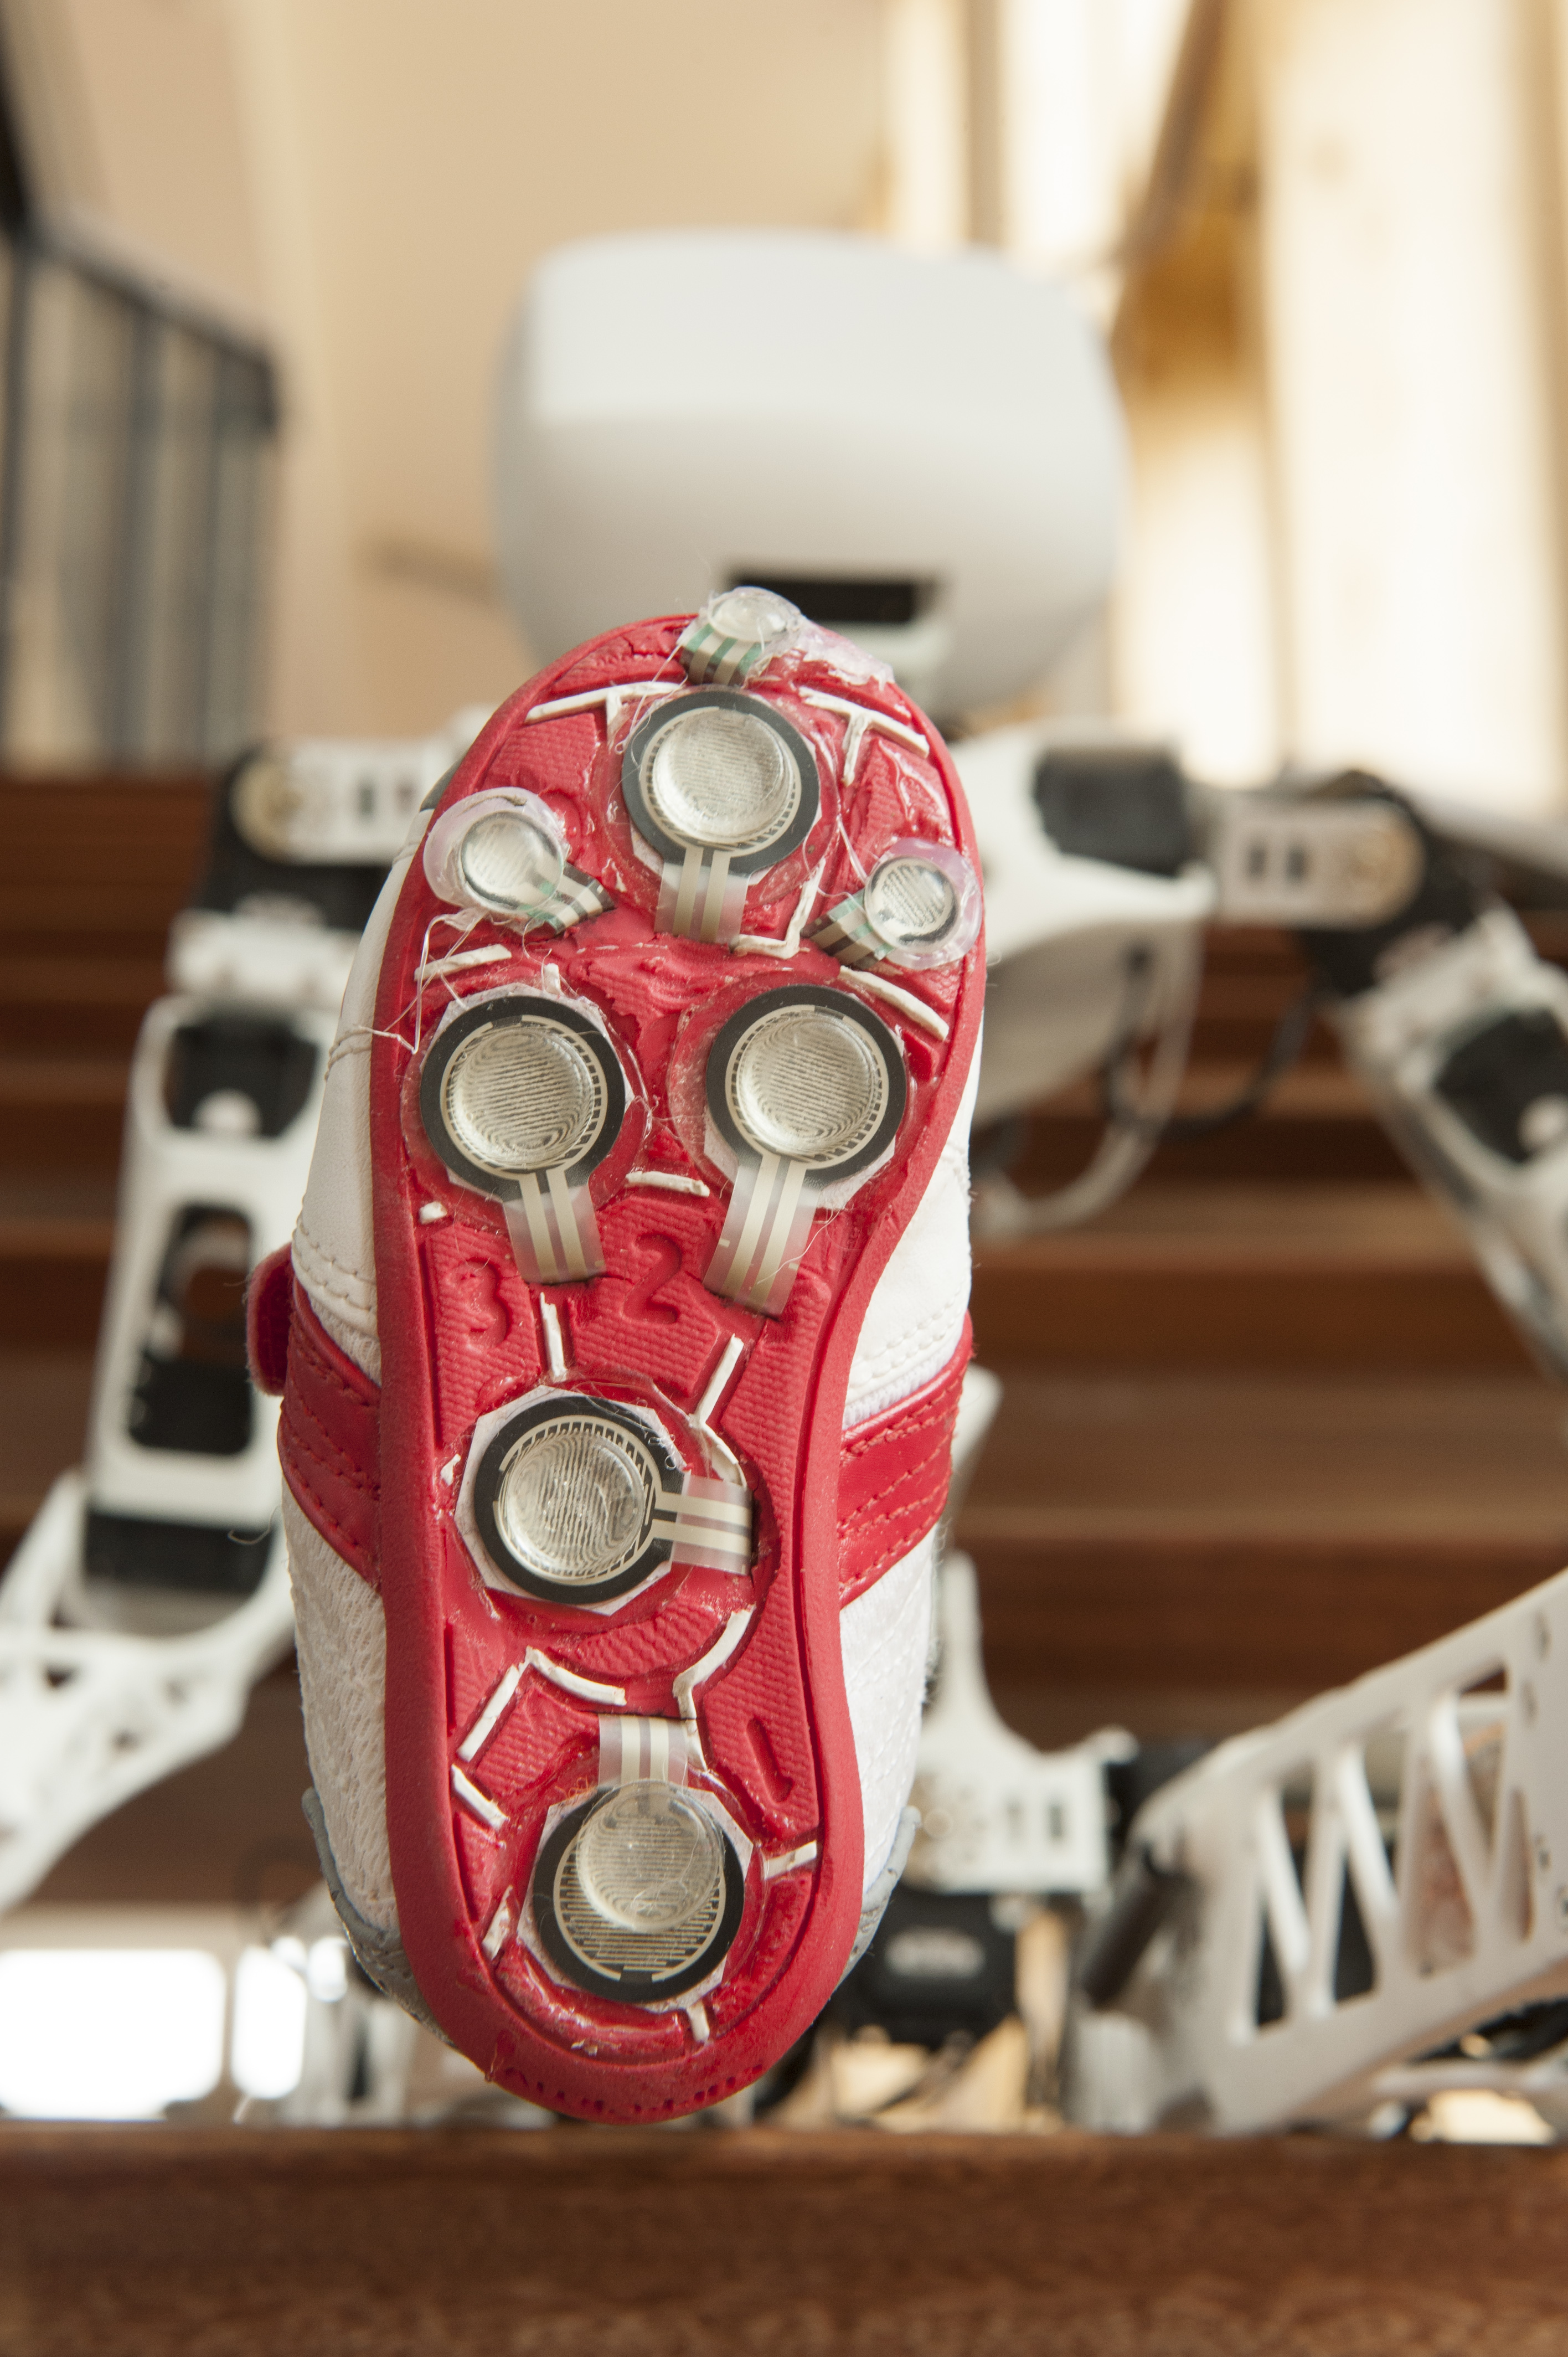
\includegraphics[height=7cm]{foot_sensors.jpg}}
    \hfil
    \subfloat[][]{\label{fig:poppy_nano_integration}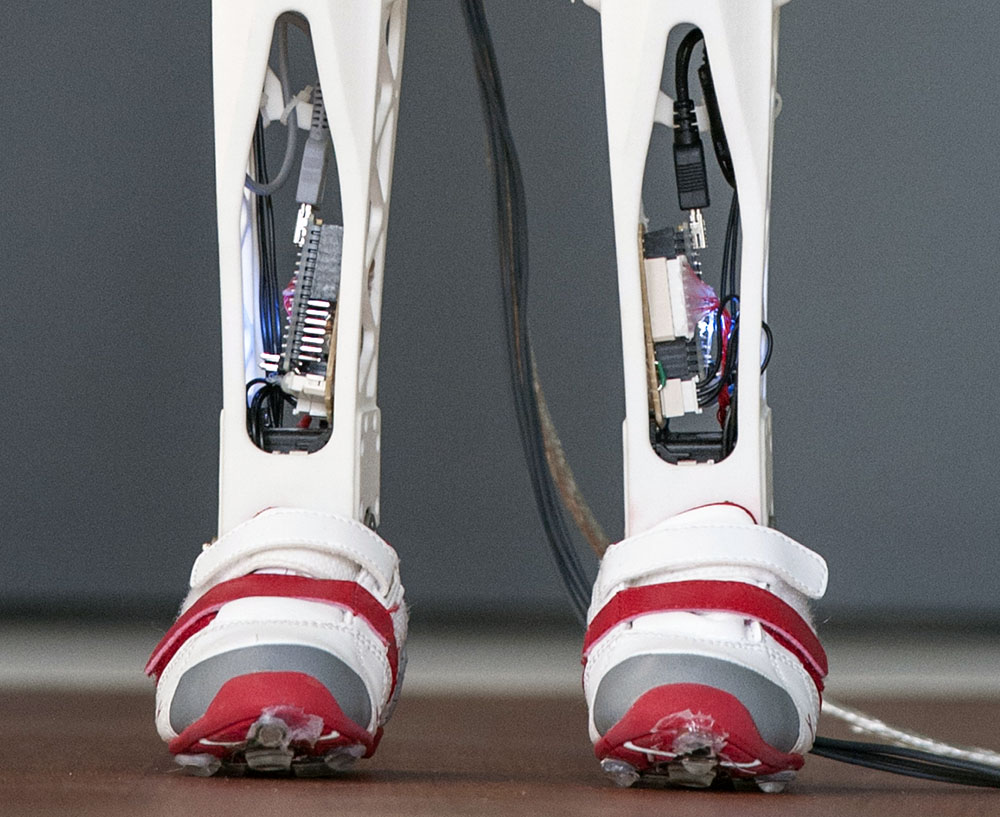
\includegraphics[height=7cm]{poppy_leg_arduino_nano.jpg}}
    \caption{}
    \label{fig:poppy_foot_sensors}
\end{figure}


As we explained in section~\ref{REF}, the Arduino programming language makes low level programming accessible to anyone. The \codename~\ref{code:arduino_foot_sensor} shows what we actually uploaded on each Arduino nano board. With just 10 lines of code we can stream the values of 5 pressure sensors.

\lstinputlisting[
    language = C++,
    caption = {Arduino code to read force sensors data},
    label = {code:arduino_foot_sensor},
    float,
    floatplacement = H]
    {code/foot_force_sensors.ino}

Then we just have to create a new sensor controller in pypot (see section~\ref{REF} for details) which describes the I/O communication and obtain the desired values (see \codename~\ref{code:pypot_foot_sensor}). Here again, the design of the pypot library makes this task easy, only 20 lines of code are required to get access to add a novel sensor and create the variable to obtain its value.

\lstinputlisting[
    language = Python,
    caption = {Example of Python code written to add custom foot sensors in pypot. The \emph{FootIO} class describes how we can read the data from the Arduino nano placed in the foot. The \emph{FootPressure} class is the sensor controller which is called by the pypot to synchronize the sensorimotor space of Poppy.},
    label = {code:pypot_foot_sensor},
    float,
    floatplacement = H]
    {code/foot_io.py}


\subsection{Measured data} % (fold)
With our new sensors, we conducted a similar walking experiment to the one explained in section~\ref{REF}, showed on the \figurename~\ref{fig:humanoids2013_cpg_on_poppy} and recorded at $50hz$ the measured force variations under Poppy's feet.

The sensors are not very precise but as we can see on \figurename~\ref{fig:poppy_GRF}, the variation of the ground reaction force (mean of the 5 force sensors) over the gait cycle has a similar M-shape as the one we can find in human gait (see \figurename~\ref{fig:human_GRF}). Also we can notice than the reaction is slightly different between the two feet (\figurename~\ref{fig:right_GRF} Vs \figurename~\ref{fig:left_GRF}).

\begin{figure}[!h]
\centering
    \subfloat[][]{\label{fig:right_GRF}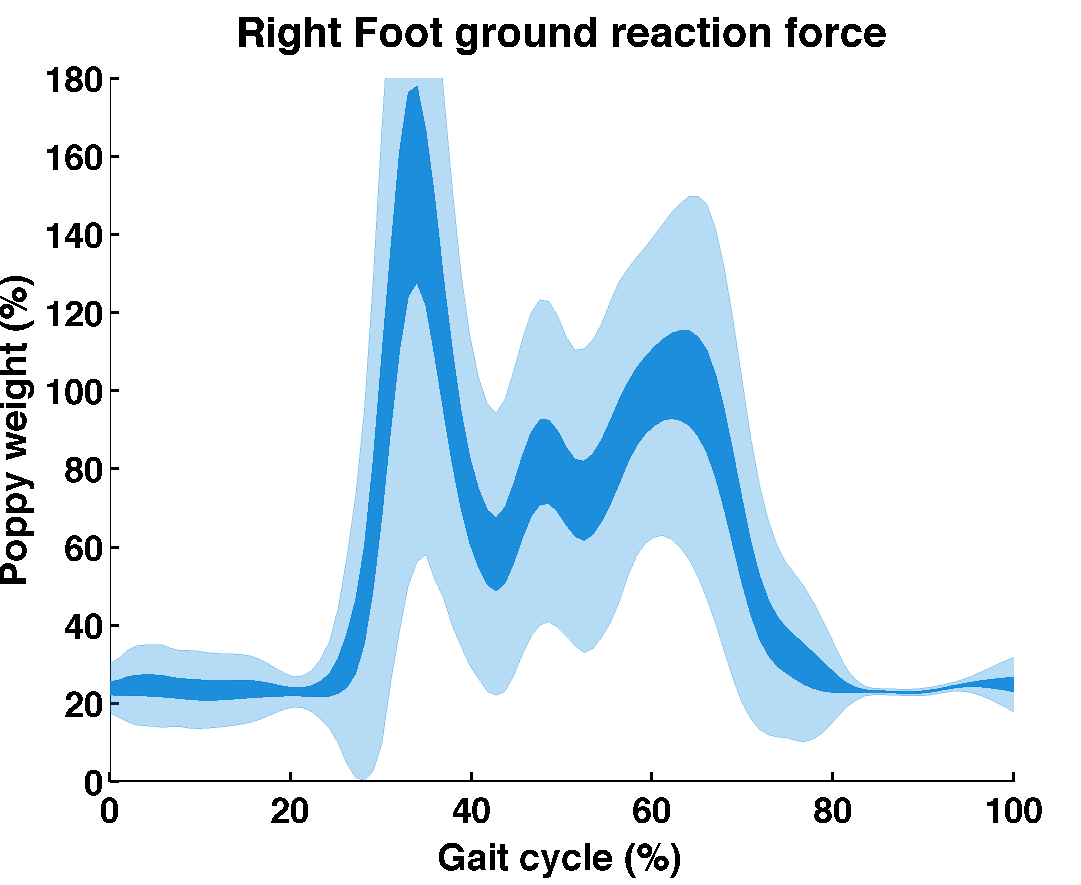
\includegraphics[width=0.48\linewidth]{right_GRF.pdf}}
    \hfil
    \subfloat[][]{\label{fig:left_GRF}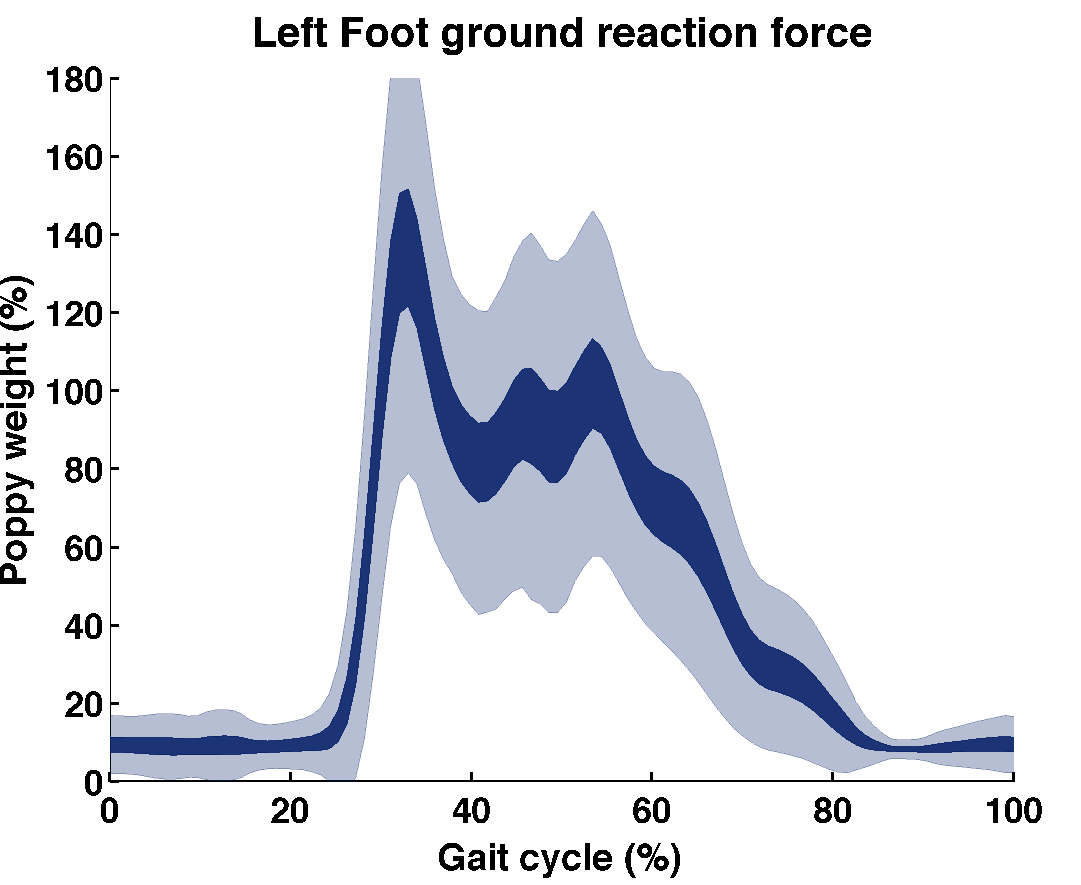
\includegraphics[width=0.48\linewidth]{left_GRF.pdf}}
    \caption{}
    \label{fig:poppy_GRF}
\end{figure}


\begin{figure}[!h]
\centering
    \subfloat[][]{\label{fig:}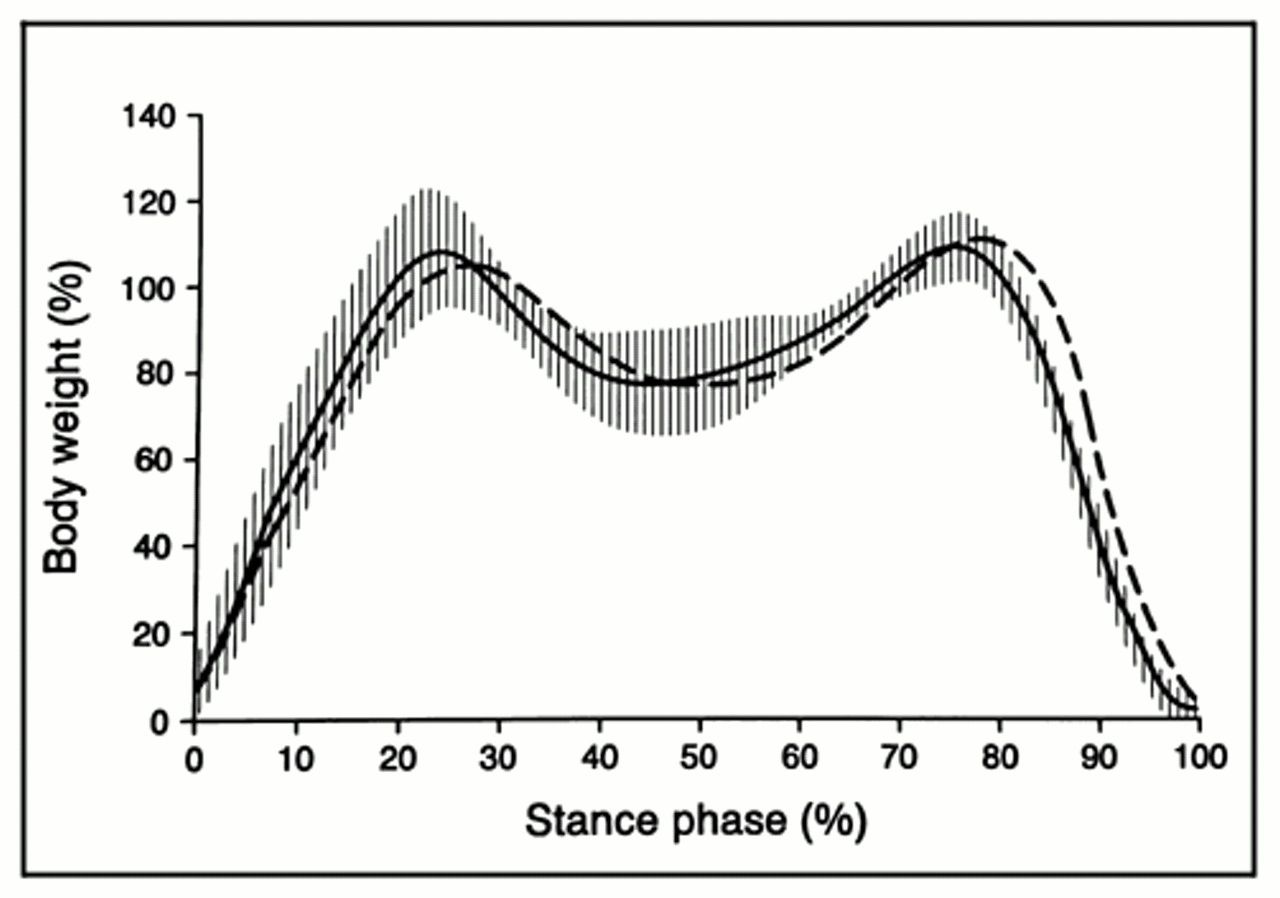
\includegraphics[width=0.6\linewidth]{human_GRF.jpg}}\newline
    \subfloat[][]{\label{fig:}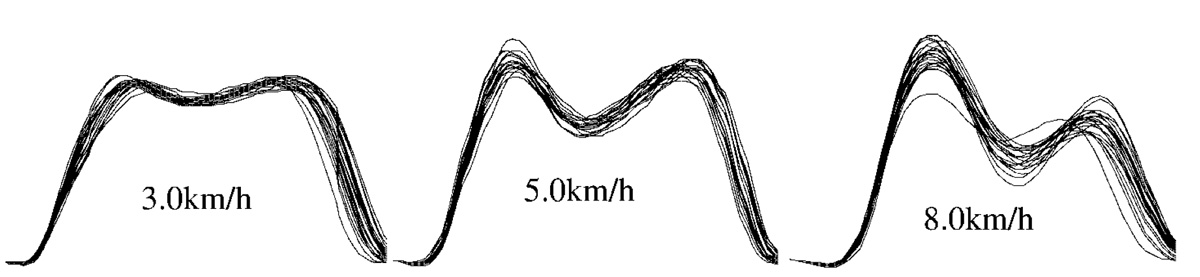
\includegraphics[width=\linewidth]{human_GRF_variation.jpg}}
    \caption{}
    \label{fig:human_GRF}
\end{figure}


The poor precision of the sensors prevents us from affirming conclusions but it can still give insights into understanding the walking behavior of Poppy:
\begin{enumerate}
    \item The second peak of the M-shape corresponding to the toe impulsion is weak or inexistent on Poppy. Indeed, when we watch the video of Poppy’s walking gait, we can see that the toes are barely used.
    \item The first peak of the M-shape is very pronounced. Either Poppy’s walking gait was fast or the structure is too rigid and does not correctly absorb the initial impact.
\end{enumerate}

We can therefore explore some avenues for improvement:
\begin{enumerate}
    \item Explore why the current walking behavior does not involve clearly the passive toes. Is this caused by the primitive walking design or the mechanical design of the toes?
    \item The initial impact is not desirable for achieving a self-balanced walking behavior. We should explore solutions to absorb it.
\end{enumerate}


